\scanpage{43}
\noindent\hfill \unsure{a}\illegible{1}n \mspage{3}

\noindent evidence of hand computed tables,was found to fail for the case of $7^{3}$ by CHOWLA(1934) who observed that $p(243)$,computed by GUPTA(1935), is not divisible by $7^{3}$. This provides a simple illustration of the value of computers; had Ramanujan lived 50 years later he would surely have tested his conjecture extensively and probably found the correct form for $7$. WATSON(1938)proved the conjecture for all powers of $5$,and a suitably modified form for all powers of $7$,while ATKIN(1967)proved the conjecture for all powers of $11$. Thus the true form of \handwritten{(2.1)} is
\[
\begin{aligned}
&\handwritten{\text{\uline{if}}\quad 24n-1\equiv0\,(\text{\uline{mod}}\;5^{a}7^{b}11^{c})\quad
\text{\uline{then}}\quad p(n)\equiv0\,(\text{\uline{mod}}\;5^{a}7^{\beta}11^{c}),}\\
&\qquad\handwritten{\text{\uline{where}}\quad \beta=[(b+2)/2].}
\end{aligned}
\tag*{\handwritten{(2.3)}}
\]

It might be argued that for Ramanujan to have obtained the correct form \handwritten{(2.3)}would have been relatively unimportant; that the \uline{idea} of such a prop\rlap{\handwritten{\tikz[baseline=0pt,x=.7em,y=1ex,line cap=round]{\draw (-.18,-.82)--(.04,-.20)--(.45,-.78);\draw (.04,.4)--(.32,1.75);}}}\inserted{\handwritten{\uline{e}}}\margin{\handwritten{\tikz[x=.32em,y=.72ex,line cap=round]{\draw (0,0)--(1.2,3.4);\draw (.25,.68).. controls (.6,1.0) and (.8,.1) ..(1.2,.1);}}}rty is all that matters short of actual proof. But this is far from true in this kind of work,since the exact numerical form of such results can often provi\rlap{\handwritten{\tikz[baseline=0pt,x=1em,y=1ex]{\draw (0,-.35)--(.56,-.35)--(.56,1.7)--(1.06,1.7);}}}ed important clues as to a possible method of proof.

Despite the early recognition of the modular nature o\deleted{\unsure{n|f}}\handwritten{f} these congruences,it was not until 1949 that LEHNER(1949a,1949b) considered the analogous properties of $c(n)$,where
\[
\handwritten{j(\tau)=j(x)=\sum_{n=-1}^{\infty}c(n)\,x^{n}
=\left\{1+240\sum_{n=1}^{\infty}\sigma_{3}(n)x^{n}\right\}^{3}\big/xf^{24}(x)-744^{*}}
\tag*{\handwritten{$\ldots$ (2.4)}}
\]

\noindent\handwritten{\rule{\linewidth}{0.4pt}}

\noindent *We choose the arbitrary constant in $j(x)$ to make $c(0)=0$ and thus avoid tiresome exceptions to our results.

\handwritten{\figure{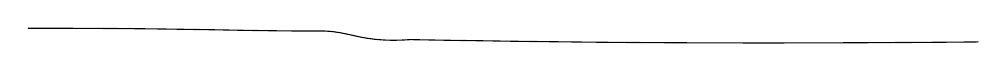
\begin{tikzpicture}[x=\linewidth,y=1mm,line cap=round]
\draw (0,.5) .. controls (.18,.5) and (.23,.1) .. (.31,.15) .. controls (.34,0) and (.35,-1.35) .. (.4,-.95) .. controls (.55,-1.25) and (.71,-1.55) .. (.995,-1.24);
\end{tikzpicture}}}

\[
\handwritten{\text{and}\qquad \sigma_{3}(n)=\sum_{d\mid n}d^{3}.}
\]

This function $j(\handwritten{\tau})$ is essentially the simplest of all modular forms, being in fact the Hauptmodul of the full modular group so that
\[
\handwritten{j\left(\frac{a\tau+b}{c\tau+d}\right)=j(\tau)\quad
\text{\uline{for} \uline{all} \uline{integral}}\quad a,b,c,d\quad
\text{\uline{with}}\quad ad-bc=1.}
\]
The results for $c(n)$ are
\[
\begin{aligned}
&\handwritten{\text{if}\quad n\equiv0\,(\mathrm{mod}\;2^{a}3^{b}5^{c}7^{d}11^{e})\quad
\text{then}\quad c(n)\equiv0\,(\mathrm{mod}\;2^{3a+8}3^{2b+3}\,\unsure{<|\hookleftarrow}}\\
&\hspace{4em}\handwritten{\unsure{>|\hookrightarrow}\,5^{c+1}7^{d}11^{e}).}
\end{aligned}
\tag*{\handwritten{(2.5)}}
\]

% archive sheet number: 42
